\documentclass[a4paper, 12pt]{article}


\usepackage{graphicx}
\usepackage{xcolor}
\usepackage{listings}

\lstset{
    language=C++,
    frame=single,
    numbers=left,
    numberstyle=\tiny\color{gray},
    numbersep=5pt,
    tabsize=4,
    basicstyle=\ttfamily\small,
    keywordstyle=\color{blue},
    commentstyle=\color{green},
    stringstyle=\color{red}
}

\begin{document}

\begin{figure}[ht]
  \begin{center}
    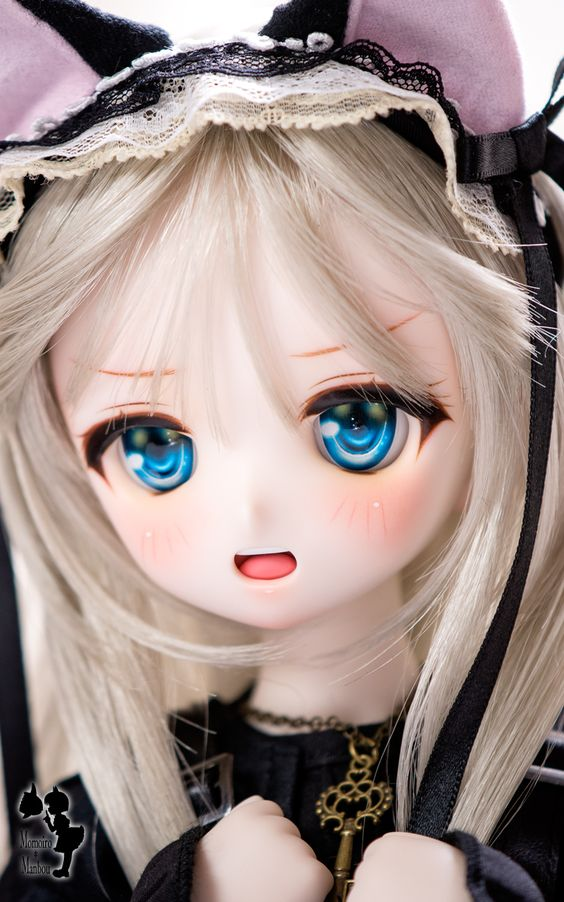
\includegraphics[width=0.8\textwidth]{./boneka.jpg}
  \end{center}
  \caption{boneka}\label{fig:boneka}
\end{figure}


\begin{lstlisting}
  #include <iostream>
  riski homosek
  int main() {
      std::cout << "Hello, world!" << std::endl;
      if shigure == 15{
      sissu homosek;
      }
      return 0;
  }
\end{lstlisting}
\end{document}
